\subsubsection{H-Brücke}
\label{subsubsec:H-Brücke}

Das Bindeglied zwischen Kraft (Motor) und Steuersignalen wird von der H-Brücke gebildet. Durch Laden-/Entladen der MOSFET-Gates wird eine Spannung an einer Spule angelegt oder weggenommen. Wie sich das Ein- und Ausschalten der einzelnen Phasenbrücken auf den Motor auswirkt, wird zu einem späteren Zeitpunkt erklärt\todo{Referenzierung auf mögliches Kapitel FOC-Steuerung mit BLDC-Motor / Reglerauslegung}. Für die Dimensionierung und Aufbau wurde das Schema vom TMC6200 als Referenzschema verwendet.\todo{Referenzierung auf TMC6200 Schemata} Die Dimensionierung der Shunts wird in Kapitel \ref{subsubsec:Gate-Treiber} abgehandelt.

\paragraph{Schaltungsaufbau}

Der Schltungsaufbau ergibt sich durch den dreiphasigen Aufbau des BLDCs. Es werden so drei Stränge gebildet, woran jeweils eine Spule verbunden wird. Der Energiefluss führt dabei über einen Strommesswiderstand. Die Eingänge der H-Brücke werden zusätlich mit Stütz- und Filterkondensatoren bestückt, um eine saubere Netzspannung zu gewährleisten.

\begin{figure}[h!]
	\centering
	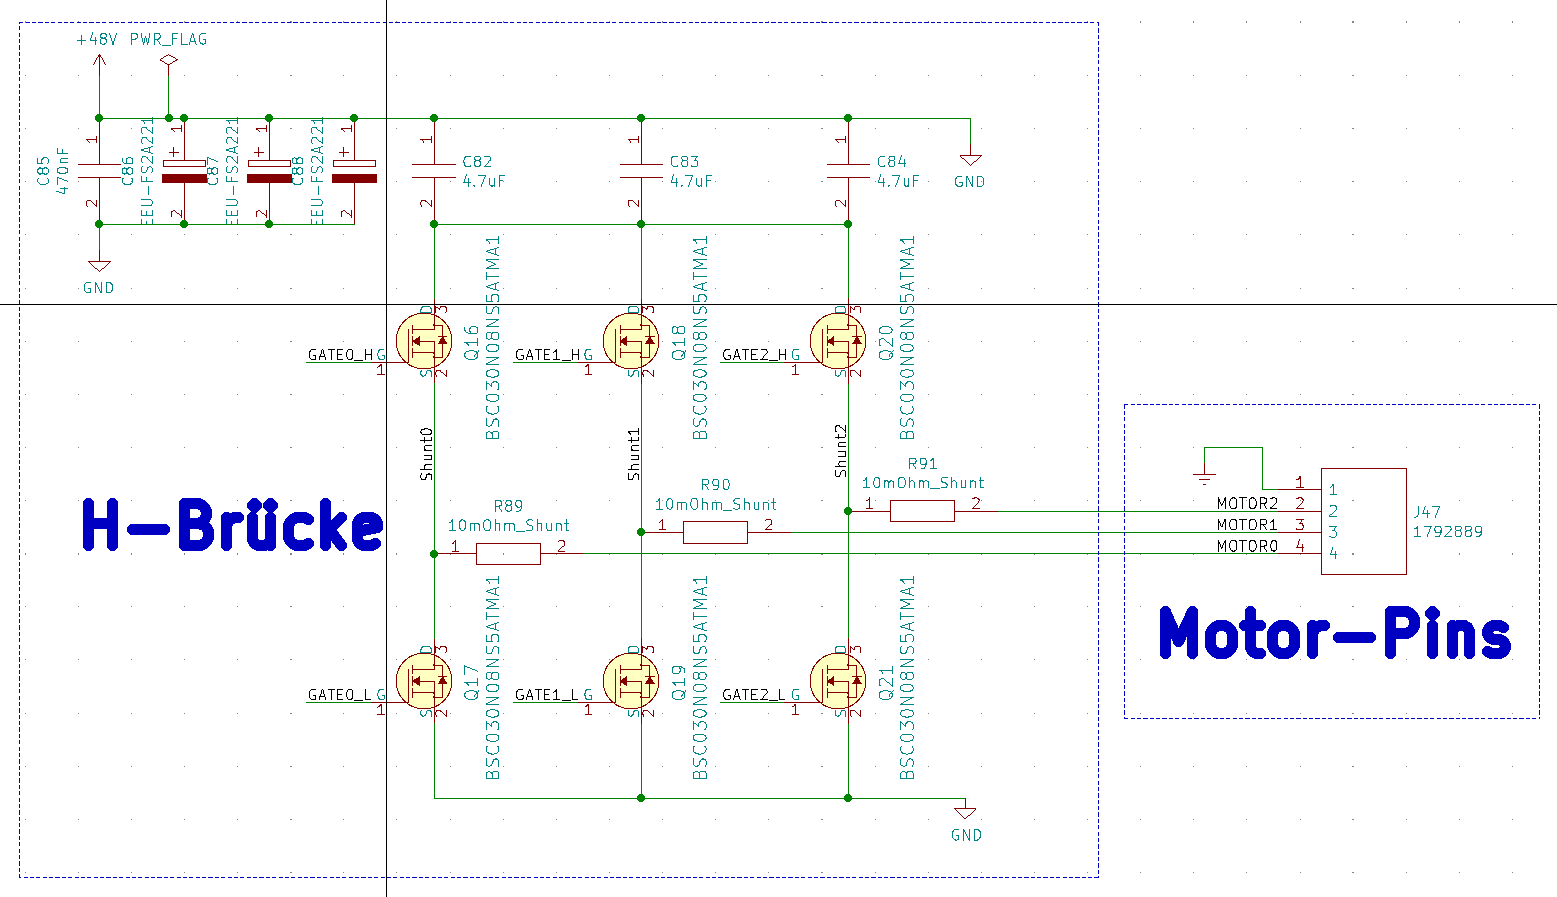
\includegraphics[width=0.7\textwidth]{graphics/Schema_H_Bruecke_und_BLDC}
	\caption{H-Brücke.}
	\label{fig:Schema_H_Bruecke_und_BLDC}
\end{figure}

\newpage

\paragraph{Funktionsbeschrieb}

C85

C86-C88

Low-ESR Stützkondensatoren für Leistungsfluss. Jeweils pro Phase einer.

C82-C84



Q16 - Q21